\section{General architecture}
The structure of the project can be best described as an implementation of the multitier architecture consisting of the Translation Memory Core, the User Space and the web application GUI, as can be seen in the figure \ref{projectStructure:layers}.

\begin{figure}[h]
\begin{center}
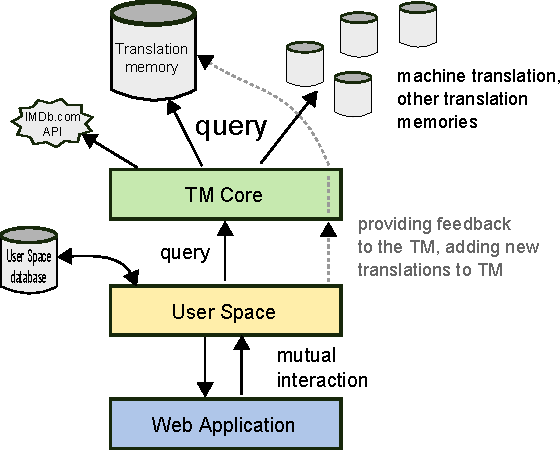
\includegraphics{figures/scheme.pdf}
\end{center}
\caption{Scheme of the application architecture.}\label{projectStructure:layers}
\end{figure}

The deepest level of the application is the Translation Memory Core which operates directly with the parallel chunks stored in database. It is implemented in Scala. It provides an interface for retrieving translation suggestions from multiple sources -- different ways of processing our own translation memory, publicly available translation memories or a machine translation output. It also assigns a score for each suggestion based on the retrieval parameters (typically the match score) and movie characteristics taken from the IMDb.com API.

The middle-ware layer is called the User Space (US). Its tasks is to interact with the translation memory itself and mirror all GUI operations on the server side. The User Space is implemented in Java. The TM Core is used only as a service which is queried for translation suggestions. The interaction with the GUI is much more complicated because each operation from GUI has to be reflected in the US. The US provides a permanent storage of users' work to make the whole application including the users data available from the Internet. Except this function the US provides the TM suggestion for the GUI and keep them up to date (the TM is gradually improving, so after a week pause in work and a subtitle file, some better sentences in TM may occur).

GUI...

\section{Logical structure of work with TM}

In this section, the general structure of work with translation memory is described, from which a design of common classes is inferred, later used both in US, GUI and Core.

Each user of the TM, except its own setting, authentication data etc., can own multiple subtitle files which we call \emph{Documents}. The documents contains information which movie whose subtitles are being translated and list of the subtitles chunks which either have been already translated or are waiting for translation.

The chunks are wrapped in to the \emph{Translation Result} objects which contains the the timed chunk from the original subtitle file, a chunk produced by the user as a translation of the original chunk, a list of translation suggestions from translation memory which are in fact.

\begin{figure}[h]
\begin{center}
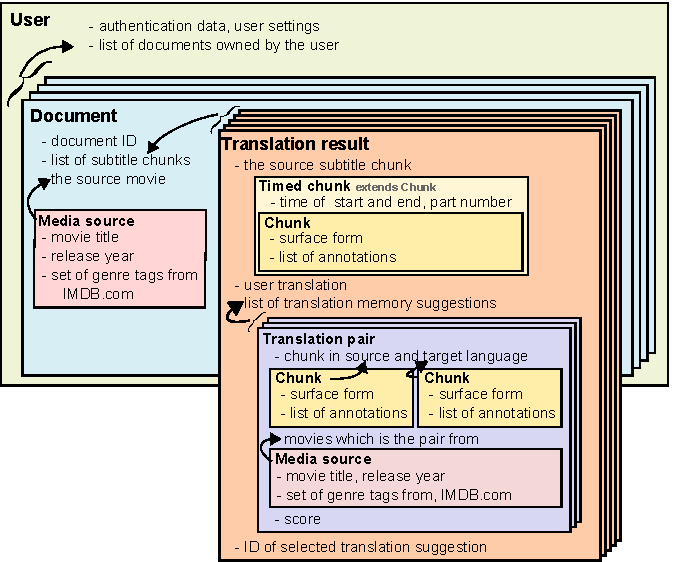
\includegraphics{figures/shared_classes.pdf}
\end{center}
\caption{Scheme of the application architecture.}\label{projectStructure:logical}
\end{figure}

All mentioned characteristics are common for both US and GUI. Because all parts of the project are Java based we can use a set of shared classes. Despite there are some limitations due to the fact that the GWT implements only a subset of Java functionality, using a shared classes structure makes the whole project clearer. 

%If we look at the structure of a document being translated which is mirrored in the GUI and in the US, we can notice there together parts originating in different part of the projects.
